% Copyright 2015--2023  Ed Bueler

\documentclass[10pt,hyperref]{beamer}

\mode<presentation>
{
  \usetheme{Madrid}

  \usecolortheme{beaver}

  \setbeamercovered{transparent}
  
  \setbeamerfont{frametitle}{size=\large}
}

\setbeamercolor*{block title}{bg=red!10}
\setbeamercolor*{block body}{bg=red!5}

\usepackage[english]{babel}
\usepackage[latin1]{inputenc}
\usepackage{times}
\usepackage[T1]{fontenc}
% Or whatever. Note that the encoding and the font should match. If T1
% does not look nice, try deleting the line with the fontenc.

\usepackage{empheq,bm,xspace,fancyvrb}
\usepackage{hyperref}

% If you wish to uncover everything in a step-wise fashion, uncomment
% the following command: 
%\beamerdefaultoverlayspecification{<+->}

\newcommand{\bb}{\mathbf{b}}
\newcommand{\bc}{\mathbf{c}}
\newcommand{\bbf}{\mathbf{f}}
\newcommand{\bl}{\bm{\ell}}
\newcommand{\br}{\mathbf{r}}
\newcommand{\bs}{\mathbf{s}}
\newcommand{\bx}{\mathbf{x}}
\newcommand{\by}{\mathbf{y}}
\newcommand{\bv}{\mathbf{v}}
\newcommand{\bu}{\mathbf{u}}
\newcommand{\bw}{\mathbf{w}}

\newcommand{\bzero}{\bm{0}}

\newcommand{\CC}{\mathbb{C}}
\newcommand{\RR}{\mathbb{R}}

\newcommand{\ddt}[1]{\ensuremath{\frac{\partial #1}{\partial t}}}
\newcommand{\ddx}[1]{\ensuremath{\frac{\partial #1}{\partial x}}}
\renewcommand{\t}[1]{\texttt{#1}}
\newcommand{\Matlab}{\textsc{Matlab}\xspace}
\newcommand{\Octave}{\textsc{Octave}\xspace}
%\newcommand{\MO}{\Matlab/\Octave}
\newcommand{\MO}{\Matlab}
\newcommand{\eps}{\epsilon}

\newcommand{\twovect}[4]{\ensuremath{{#1}_{#2} =
                            \begin{bmatrix} #3 \\ #4 \end{bmatrix}}}

\newcommand{\mfile}[1]{
\VerbatimInput[frame=single,label=\fbox{\scriptsize \textsl{\,#1\,}},fontfamily=courier,fontsize=\scriptsize]{#1}
}

\newcommand{\mfiletiny}[1]{
\VerbatimInput[frame=single,label=\fbox{\scriptsize \textsl{\,#1\,}},fontfamily=courier,fontsize=\tiny]{#1}
}


\title[Classical iterative methods]{Classical iterative methods \\ for linear and nonlinear systems}

\author{Ed Bueler}

\institute[MATH 615 NADE]{MATH 615 Numerical Analysis of Differential Equations}

\date{Spring 2023}

\AtBeginSection[]
{
  \begin{frame}<beamer>
    \frametitle{Outline}
    \tableofcontents[currentsection,hideallsubsections]
  \end{frame}
}

\begin{document}

\begin{frame}
  \maketitle
\end{frame}


\begin{frame}{example linear systems}

\begin{itemize}
\item suppose we want to solve the linear system
\begin{equation}
A \bx = \bb \label{introsystem}
\end{equation}
where $A\in \RR^{m\times m}$ and $\bb\in \RR^m$
\item the goal is to find $\bx\in \RR^m$
\item  throughout these notes we use 2 linear system examples:
  \begin{itemize}
  \item[LS1] 
\begin{equation*}
\begin{bmatrix} 2 & 1 & 0 \\
                0 & 2 & 1 \\
                1 & 0 & 3 \end{bmatrix}
\begin{bmatrix} x_1 \\ x_2 \\ x_3 \end{bmatrix}
=
\begin{bmatrix} 2 \\ 1 \\ 4 \end{bmatrix}
\end{equation*}
  \item[LS2]
\begin{equation*}
\begin{bmatrix} 1 & 2 & 3 & 0 \\
                2 & 1 &-2 &-3 \\
               -1 & 1 & 1 & 0 \\
                0 & 1 & 1 &-1 \end{bmatrix}
\begin{bmatrix} x_1 \\ x_2 \\ x_3 \\ x_4 \end{bmatrix}
=
\begin{bmatrix} 7 \\ 1 \\ 1 \\ 3 \end{bmatrix}
\end{equation*}
  \end{itemize}
\item it is trivial to find solutions of LS1, LS2 using the ``\texttt{x=A$\backslash$b}'' black box in \Matlab (or similar)
\item LS1 and LS2 stand-in for the large linear systems we get from applying finite difference (FD) schemes to ODE and PDE problems
\end{itemize}
\end{frame}


\begin{frame}{residual}

\begin{itemize}
\item the \emph{residual} of a vector $\bv$ in linear system \eqref{introsystem} is the vector
\begin{equation}
\br(\bv) = \bb - A \bv \label{residualdefn}
\end{equation}
\item making the residual zero is the same as solving the system:
      $$A \bx=\bb \, \iff \, \br(\bx)=0$$
\item evaluating $\br(\bv)$ needs a matrix-vector product and a vector subtraction
  \begin{itemize}
  \item[$\circ$] requires $O(m^2)$ operations at worst
  \item[$\circ$] by comparison, applying Gauss elimination to solve linear system \eqref{introsystem} is an $O(m^3)$ operation in general
  \end{itemize}
\end{itemize}
\end{frame}


\begin{frame}{sparse matrices}

\begin{itemize}
\item \emph{definition.}  a matrix with enough zeros to allow exploitation of that fact is called \emph{sparse}
  \begin{itemize}
  \item[$\circ$] the figure shows \texttt{spy} plots of 3 matrices; nonzero entries are in black
  \item[$\circ$] numerical schemes for differential equations generate matrices $A$ for which the majority, often $99\%$ or more, of the entries are zero
  \end{itemize}
\item a non-sparse matrix is called \emph{dense}, e.g.~when most entries are nonzero
  \begin{itemize}
  \item[$\circ$] even if $A$ is sparse, $A^{-1}$ is generally dense
  \end{itemize}
\item evaluating the residual of a sparse matrix with at most $z$ nonzero entries per row requires $O(m)$ operations
  \begin{itemize}
  \item[$\circ$] specifically, at most $(2z+1)m$ operations
  \end{itemize}
\end{itemize}

\bigskip
\begin{center}
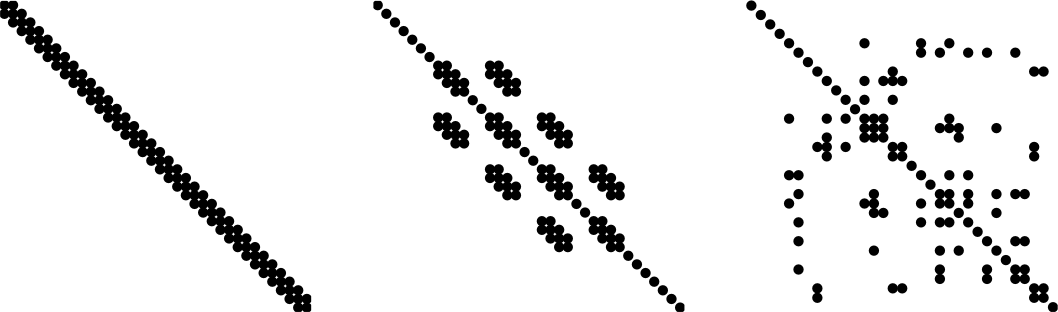
\includegraphics[width=0.7\textwidth]{sparsities.png}
\end{center}
\end{frame}


\begin{frame}{Richardson iteration}

\begin{itemize}
\item \emph{iterative methods} for the linear system $A\bx=\bb$ attempt to solve it based only on computing the residual or applying $A$ to a vector
  \begin{itemize}
  \item[$\circ$] one wants the sequence of approximations, the iterates, to \emph{converge} to the solution $\bx = A^{-1} \bb$
  \item[$\circ$] Iterative methods always require an initial iterate $\bx_0$
  \end{itemize}
\item for example, \emph{Richardson iteration} adds a multiple $\omega$ of the last residual at each step:
\begin{equation}
\bx_{k+1} = \bx_k + \omega (\bb - A \bx_k)  \label{richardson}
\end{equation}
\item for system LS1, using initial iterate $\bx_0=0$ and $\omega=1/5$, Richardson gives:\small
\begin{align*}
\bx_0 &= \begin{bmatrix} 0 \\ 0 \\ 0 \end{bmatrix}, \,
\bx_1 = \begin{bmatrix} 0.4 \\ 0.2 \\ 0.8 \end{bmatrix}, \,
\bx_2 = \begin{bmatrix} 0.6 \\ 0.16 \\ 1.04 \end{bmatrix}, \,
\bx_3 = \begin{bmatrix} 0.728 \\ 0.088 \\ 1.096 \end{bmatrix}, \, \dots, \,
\bx_{10} = \begin{bmatrix} 0.998 \\ -0.017 \\ 1.01 \end{bmatrix},
\dots
\end{align*}
these iterates seem to be converging to $\bx = [1 \,\, 0 \,\, 1]^\top$, the solution to LS1
\item when does Richardson iteration work?
\end{itemize}
\end{frame}


\begin{frame}{recall: eigenvalues and vectors}

\begin{itemize}
\item a complex number $\lambda \in \CC$ is an \emph{eigenvalue} of a square matrix $B\in\RR^{m\times m}$ if there is a nonzero vector $\bv\in\CC^m$ so that $B \bv = \lambda \bv$
  \begin{itemize}
  \item[$\circ$] $\lambda$ is a root of a polynomial
  \item[$\circ$] even if $B$ is a real matrix, $\lambda$ may be complex
  \item[$\circ$] if $\lambda$ is complex and $B$ is real then $\bv$ must be complex
  \end{itemize}
\item the set of all eigenvalues of $B$ is the \emph{spectrum} $\sigma(B)$ of $B$
\item the \emph{spectral radius} $\rho(B)$ is the largest absolute value of an eigenvalue:
    $$\rho(B) = \max_{\lambda\in\sigma(B)}  |\lambda|$$

  \begin{itemize}
  \item[$\circ$] fact: $\rho(B) \le \|B\|$ in any induced matrix norm
  \end{itemize}
\end{itemize}
\end{frame}


\begin{frame}{spectral properties and convergence of iterations}

\begin{itemize}
\item properties of a matrix $B$ which can be described in terms of eigenvalues are generically called \emph{spectral properties}
\item some examples:
  \begin{itemize}
  \item[$\circ$] the spectral radius $\rho(B)$ itself
  \item[$\circ$] the 2-norm $\|B\|_2 = \sqrt{\rho(B^\top B)}$
  \item[$\circ$] the 2-norm condition number $\kappa(B)=\|B\|_2 \|B^{-1}\|_2$
  \end{itemize}

\medskip
\item a general idea:
\begin{quote}
whether an iterative method for solving a linear system $A\bx = \bb$ converges, or not, depends on the spectral properties of $A$, or on the spectral properties of matrices built from $A$
\end{quote}

\medskip
\item the right-hand side $\bb$ in the linear system $A\bx = \bb$, and the initial iterate $\bx_0$, generally \emph{do not} determine whether an iteration converges
  \begin{itemize}
  \item[$\circ$] a good choice of $\bx_0$ \emph{can} speed up convergence when it happens
  \end{itemize}
\end{itemize}
\end{frame}


\begin{frame}{convergence of the Richardson iteration}

\begin{itemize}
\item the Richardson iteration \eqref{richardson} can be rewritten as
    $$\bx_{k+1} = (I - \omega A) \bx_k + \omega \bb$$

\vspace{-2mm}
  \begin{itemize}
  \item[$\circ$] confirm this!
  \end{itemize}
\item Richardson iteration converges if and only if all the eigenvalues of the matrix $I-\omega A$ are inside the unit circle:

$$\text{Richardson converges if and only if } \rho(I-\omega A) < 1$$

  \begin{itemize}
  \item[$\circ$] see the lemma on the next slide
  \item[$\circ$] note $\rho(I-\omega A) < 1$ means $(I - \omega A) \bx_k$ is smaller in magnitude than $\bx_k$
  \item[$\circ$] fact: \emph{if} $\|I-\omega A\| < 1$ \emph{then} Richardson converges
  \end{itemize}
\end{itemize}
\end{frame}


\begin{frame}{convergence lemma for linear iterations}

\begin{lemma}
   $$\by_{k+1} = M \by_k + \bc$$
converges to the solution of $\by = M \by + \bc$ for all initial $\by_0$ if and only if
   $$\rho(M) < 1.$$
\end{lemma}

\small
\begin{proof}
Iterate.  That is, write out a few cases:
\begin{align*}
   \by_2 &= M (M \by_0 + \bc) + \bc = M^2 \by_0 + (I + M) \bc, \\
   \by_3 &= M (M^2 \by_0 + (I + M) \bc) + \bc = M^3 \by_0 + (I + M + M^2) \bc,
\end{align*}
and so on.  By induction we get $\by_k = M^k \by_0 + p_k(M) \bc$ where $p_k(x) = 1 + x + x^2 + \dots$ $+ x^{k-1}$.  But $p_k(x) \to 1/(1-x)$ as $k\to\infty$ iff $x\in(-1,1)$; it is a convergent Maclaurin series on that open interval.  Also, $\rho(M)<1$ iff $M^k \to 0$.  Thus $\by_k \to (I-M)^{-1} \bc$ iff $\rho(M) < 1$.
\end{proof}
\end{frame}


\begin{frame}[fragile]{convergence of the Richardson iteration 2}

\begin{itemize}
\item since the Richardson iteration converges iff $\rho(I - \omega A)<1$, we should choose $\omega$ based on the principle that
    $$\omega A \text{ should be close to the identity } I$$
\vspace{-5mm}
  \begin{itemize}
  \item[$\circ$] often not possible!
  \end{itemize}

\medskip
\item in small cases we can graph $f(\omega) = \rho(I-\omega A)$:

\medskip
\begin{columns}
\begin{column}{0.5\textwidth}
\footnotesize
\begin{verbatim}
   omega = -1:.01:1;
   rho = zeros(size(omega));
   for j = 1:length(omega)
       M = eye(n) - omega(j) * A;
       rho(j) = max(abs(eig(M)));
   end
   plot(omega,rho)
\end{verbatim}

\smallskip
\begin{itemize}
\footnotesize
\item[for LS1:]  $\rho(I - \omega A)$ dips below $1$ for $0 < \omega \lesssim 0.6$
\item[for LS2:]  $\rho(I - \omega A) \ge 1$ always
\end{itemize}
\end{column}

\begin{column}{0.4\textwidth}
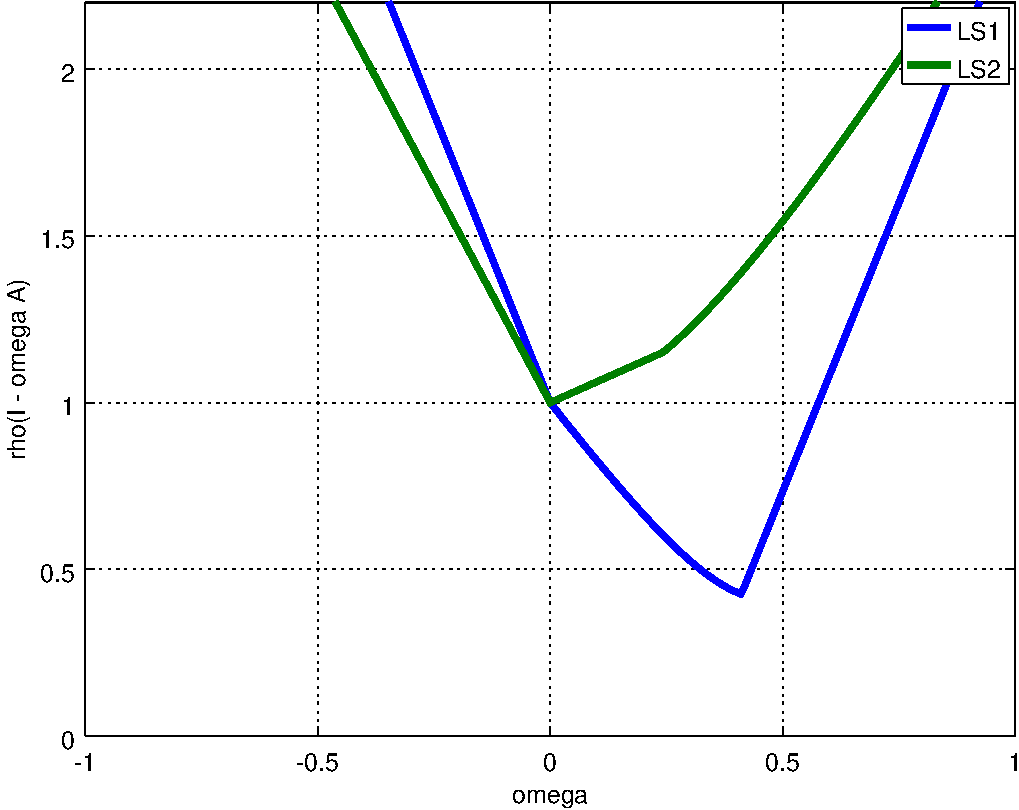
\includegraphics[width=2.0in,keepaspectratio=true]{richardspect}
\end{column}
\end{columns}

\medskip
\item  note $\rho(I-0A)=1$ \, \dots \, so no convergence when $\omega \approx 0$
\item  for LS1, figure suggests $\omega \approx 0.4$ gives fastest convergence
\end{itemize}
\end{frame}


\begin{frame}{matrix splitting}

\begin{itemize}
\item several classical iteration methods ``split'' the matrix $A$ before iterating
  \begin{itemize}
  \item[$\circ$] Richardson iteration is an exception
  \end{itemize}
\item the best known, and simplest, iteration based on splitting is \emph{Jacobi iteration}, which extracts and inverts the diagonal of $A$
\item the splitting we consider is
    $$A = D - L - U \vspace{-3mm}$$
where
  \begin{itemize}
  \item[$\circ$] $D$ is the diagonal of $A$
  \item[$\circ$] $L$ is strictly lower triangular ($\ell_{ij} = 0$ if $i \le j$)
  \item[$\circ$] $U$ is strictly upper triangular ($u_{ij} = 0$ if $i \ge j$)
  \end{itemize}
\item you can split \emph{any} matrix this way
\item see section 4.2 of the textbook

\medskip
\item so that $D$ is an invertible matrix, for the remaining slides we assume

\centerline{\emph{all diagonal entries of $A$ are nonzero}: \quad  $a_{ii} \ne 0$}
\end{itemize}
\end{frame}


\begin{frame}{Jacobi iteration}

\begin{itemize}
\item the Jacobi iteration is
\begin{equation}
D \bx_{k+1} = \bb + (L + U) \bx_k  \label{jacobi}
\end{equation}
\item if it converges then $D\bx = \bb + (L+U)\bx$, which is the same as $A \bx = \bb$
\item we could also write it as \quad $\bx_{k+1} = D^{-1} \left(\bb + (L + U) \bx_k\right)$ \quad or as
\begin{equation}
x_i^{(k+1)} = \frac{1}{a_{ii}} \left(b_i - \sum_{j\ne i} a_{ij} x_j^{(k)}\right)  \label{jacobiA}
\end{equation}
where $x_j^{(k)}$ denotes the $j$th entry of the $k$th iterate $\bx_k$

\medskip
\item make sure you understand why \eqref{jacobi} and \eqref{jacobiA} are the same!
\end{itemize}
\end{frame}


\begin{frame}{Gauss-Seidel iteration}

\begin{itemize}
\item \emph{Gauss-Seidel iteration} instead extracts and inverts the non-strict lower-triangular part of $A$
\item if $A = D - L - U$ then Gauss-Seidel is
\begin{equation}
(D - L) \bx_{k+1} = b + U \bx_k  \label{gaussseidel}
\end{equation}

\vspace{-2mm}
  \begin{itemize}
  \item[$\circ$] we could also write it as ``\,$\bx_{k+1} = (D-L)^{-1} \left(b + U \bx_k\right)$\,'', but \emph{don't} \dots that would miss the point!
  \end{itemize}
\item instead we write it as \quad $D \bx_{k+1} = b + U \bx_k + L \bx_{k+1}$ \quad or equivalently:
\begin{equation}
x_i^{(k+1)} = \frac{1}{a_{ii}} \left(b_i - \sum_{j > i} a_{ij} x_j^{(k)} - \sum_{j < i} a_{ij} x_j^{(k+1)}\right)  \label{gaussseidelA}
\end{equation}
\item the lower-triangular entries of $A$ apply to \emph{those entries of $\bx_{k+1}$ which have already been computed}
\item form \eqref{gaussseidelA} is actually \emph{easier} to implement than Jacobi \eqref{jacobiA}  \quad (why?)
\end{itemize}
\end{frame}


\begin{frame}{convergence conditions for Jacobi and Gauss-Seidel}

\begin{itemize}
\item the convergence lemma says that
  \begin{itemize}
  \item[$\circ$] Jacobi iteration converges if and only if $\rho(D^{-1} (L+U)) < 1$
  \item[$\circ$] Gauss-Seidel iteration converges if and only if $\rho((D-L)^{-1} U) < 1$
  \end{itemize}
\item these conditions are hard to use in practice because computing a spectral radius can be just as hard as solving the original system
\end{itemize}
\end{frame}


\begin{frame}{diagonally-dominant matrices}

\begin{itemize}
\item \emph{definition}.  $A$ is \emph{strictly diagonally-dominant} (SDD) if $|a_{ii}| > \sum_{j\ne i} |a_{ij}|$
  \begin{itemize}
  \item[$\circ$] $A$ in LS1 is SDD
  \item[$\circ$] $A$ in LS2 is not
  \item[$\circ$] SDD is a common, but not universal, property of the matrices coming from FD schemes on ODEs and PDEs
  \end{itemize}

\item facts:\footnote{section 11.2 of Golub and van Loan, \emph{Matrix Computations}, 4th edition 2013}
  \begin{itemize}
  \item[$\circ$] if $A$ is strictly diagonally-dominant then both the Jacobi and Gauss-Seidel iterations converge; see problem \textbf{P14} 
  \item[$\circ$] if $A$ is symmetric positive definite then Gauss-Seidel iteration converges
  \item[$\circ$] these are only \emph{sufficient} conditions, e.g.~there are nonsymmetric $A$, which are \emph{not} diagonally-dominant, for which the iterations converge
  \end{itemize}
\item unlike the ``$\rho(\dots) < 1$'' conditions on the last slide, it is easy to check SDD
\end{itemize}
\end{frame}


\begin{frame}{\emph{interlude:} past and future}

\begin{itemize}
\item the Jacobi and Gauss-Seidel iterations are from the 19th century
\item Richardson iteration first appears in a 1910 publication
\item the early history of numerical partial differential equations, e.g.~in the 1920 to 1970 period, heavily used these classical iterations
  \begin{itemize}
  \item[$\circ$] a generalization of Gauss-Seidel iteration called \emph{successive over-relaxation}, was a particular favorite around 1970;  see section 4.2 of the textbook
  \end{itemize}
\item none of these iterations work on system LS2
\item there are better iterative ideas; they flourished starting in the 1980-90s
  \begin{itemize}
  \item[$\circ$] among the best known are CG = \emph{conjugate gradients} ($\sim$1950) and GMRES = \emph{generalized minimum residuals} (Saad and Schultz, 1986)
  \item[$\circ$] GMRES works (i.e.~converges at some rate) on LS2
  \item[$\circ$] \emph{but} there is no ``good iteration'' with a universally-fast convergence rate for all matrices\footnote{a remarkable 1992 theorem by Nachtigal, Reddy, and Trefethen}
  \end{itemize}
\item iterative methods for solving linear systems will dominate the future:
  \begin{itemize}
  \item[$\circ$] they are obligatory on sufficiently-big systems
  \item[$\circ$] they work better in parallel than direct methods like Gauss elimination
  \item[$\circ$] they can exploit partial knowledge of the underlying model/question
  \end{itemize}
\end{itemize}
\end{frame}


\begin{frame}{\emph{interlude:} biographies}

\begin{itemize}
\small
\item of course, Gauss (1777--1855) did lots of big stuff:

    \centerline{\href{https://en.wikipedia.org/wiki/Carl_Friedrich_Gauss}{\texttt{en.wikipedia.org/wiki/Carl\_Friedrich\_Gauss}}}

\medskip
\item Jacobi (1804--1851) also has his name on the ``Jacobian'', the matrix of derivatives appearing in Newton's method for systems of equations:

    \centerline{\href{https://en.wikipedia.org/wiki/Carl_Gustav_Jacob_Jacobi}{\texttt{en.wikipedia.org/wiki/Carl\_Gustav\_Jacob\_Jacobi}}}

\medskip
\item Seidel (1821--1896) is relatively little known:

    \centerline{\href{https://en.wikipedia.org/wiki/Philipp_Ludwig_von_Seidel}{\texttt{en.wikipedia.org/wiki/Philipp\_Ludwig\_von\_Seidel}}}

\medskip
\item Richardson (1881--1953) is the most interesting.  He invented numerical weather forecasting, doing it by-hand for fun during WWI.  Later, as a pacifist and quaker, he quit the subject when he found his meteorological work was being used by chemical weapons engineers and the military:

    \centerline{\href{https://en.wikipedia.org/wiki/Lewis_Fry_Richardson}{\texttt{en.wikipedia.org/wiki/Lewis\_Fry\_Richardson}}}
\end{itemize}
\end{frame}


\begin{frame}{nonlinear systems}
\begin{itemize}
\item generally, systems of equations are \emph{not} linear, so they cannot be written in the form $A \bx = \bb$
\item instead, we can write any square system of equations using a function $\bbf:\RR^n\to \RR^n$:
    $$\bbf(\bx)=\bzero$$

  \begin{itemize}
  \item[$\circ$] ``square'' simply means the number of unknowns (inputs to $\bbf$) equals the number of equations (outputs from $\bbf$)
  \end{itemize}
\item if $\bbf$ is smooth then its first derivative is a matrix-valued function called the \emph{Jacobian} of $\bbf$:
	$$J_{ij} = \frac{\partial f_i}{\partial x_j}$$

  \begin{itemize}
  \item[$\circ$] for each $\bx$, $J(\bx)$ is an $n\times n$ matrix
  \end{itemize}
\item \emph{example}: a function and its Jacobian:
    $$\bbf(\bx) = \begin{bmatrix} \frac{1}{2} e^{2x_1} - x_2 \\ \\ x_1^2 + x_2^2 - 1 \end{bmatrix}, \qquad
    J(\bx) = \begin{bmatrix} e^{2x_1} & -1 \\ \\
                             2 x_1 & 2 x_2 \end{bmatrix}$$
\end{itemize}
\end{frame}


\begin{frame}{example of a nonlinear system}

\begin{columns}
\begin{column}{0.55\textwidth}
\begin{itemize}
\item here is an example of a nonlinear system with $\bbf:\RR^2\to\RR^2$
\item find where the circle of radius 1 intersects the graph of an exponential:
\begin{align*}
x^2+y^2 = 1 \\
y = \tfrac{1}{2} e^{2x}
\end{align*}

  \begin{itemize}
  \item[$\circ$] note there are two intersection points
  \item[$\circ$] I \emph{don't} know how to find them by hand
  \end{itemize}
\item renaming $x=x_1,y=x_2$ allows us to write this as $\bbf(\bx)=\bzero$:
  $$\bbf(\bx) = \begin{bmatrix} \frac{1}{2} e^{2x_1} - x_2 \\ \\ x_1^2 + x_2^2 - 1 \end{bmatrix}$$

  \begin{itemize}
  \item[$\circ$] the same example as on the last slide
  \end{itemize}
\end{itemize}
\end{column}
\begin{column}{0.45\textwidth}
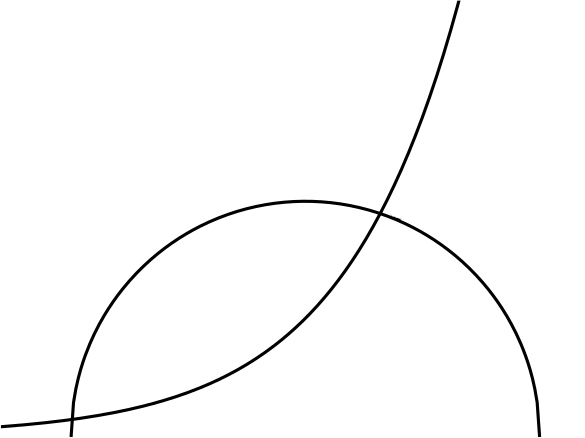
\includegraphics[width=\textwidth]{nonlinexample.png}
\end{column}
\end{columns}
\end{frame}


\begin{frame}{Newton's method}
\begin{itemize}
\item our classical linear iterations generated sequences $\bx_k$ which solved $\br(\bx) = \bb - A \bx = 0$, that is, so that $\br(\bx_k) \to \bzero$
\item similarly, \emph{Newton's method} for a system of nonlinear equations generates a sequence $\bx_k$ so that $\bbf(\bx_k) \to \bzero$

  \begin{itemize}
  \item[$\circ$] as usual, an initial iterate $\bx_0$ is needed
  \end{itemize}
\item it repeatedly linearizes $\bbf(\bx)=0$; one needs to solve a linear system to get each new iterate $\bx_k$
\item it is often surprisingly fast!
\item Newton's method:
\begin{gather}
J(\bx_k)\, \bs = - \bbf(\bx_k), \label{stepeqn} \\
\bx_{k+1} = \bx_k + \bs \label{updateeqn}
\end{gather}

  \begin{itemize}
  \item[$\circ$] eqn \eqref{stepeqn} is a system of linear equations which determines the \emph{step} $\bs$
  \item[$\circ$] eqn \eqref{updateeqn} takes the step to the next iterate
  \end{itemize}
\end{itemize}
\end{frame}


\begin{frame}{explanation of Newton's method}
\begin{itemize}
\item suppose $\bx_k$ is a current estimate of the solution $\bbf(\bx)=\bzero$
\item now linearize $\bbf$ around $\bx_k$ using Taylor's theorem with remainder:
    $$\bbf(\bx) = \bbf(\bx_k) + J(\bx_k) (\bx - \bx_k) + O(h^2)$$
where $h=\|\bx-\bx_k\|$ is the distance between the basepoint $\bx_k$ and another value $\bx$
\item the linearization of $\bbf$ comes from dropping the $O(h^2)$ term:
    $$\bl(\bx) = \bbf(\bx_k) + J(\bx_k) (\bx - \bx_k)$$
\item now define the next iterate $\bx_{k+1}$ as the zero of the linearization $\bl$:
    $$\bzero = \bbf(\bx_k) + J(\bx_k) (\bx_{k+1} - \bx_k)$$
\item denote the difference $\bx_{k+1} - \bx_k$ by $\bs$, and thus get the previous form:
\begin{gather*}
J(\bx_k)\, \bs = - \bbf(\bx_k), \\
\bx_{k+1} = \bx_k + \bs
\end{gather*}
\end{itemize}
\end{frame}


\begin{frame}{example}
\begin{columns}
\begin{column}{0.65\textwidth}
\begin{itemize}
\item recall the example, where a circle intersects an exponential: $x^2+y^2 = 1, \, y = \tfrac{1}{2} e^{2x}$
\item this nonlinear residual function and Jacobian:
{\small
    $$\bbf(\bx) = \begin{bmatrix} \frac{1}{2} e^{2x_1} - x_2 \\ \\ x_1^2 + x_2^2 - 1 \end{bmatrix}, \,
    J(\bx) = \begin{bmatrix} e^{2x_1} & -1 \\ \\
                             2 x_1 & 2 x_2 \end{bmatrix}$$
}
\item for example, run Newton's method starting from $\bx_0 = (1,1)$:
{\small
\begin{gather*}
\twovect{\bx}{0}{1}{1}, \, \twovect{\bx}{1}{0.619203}{0.880797}, \, \twovect{\bx}{2}{0.394157}{0.948623},\\
\twovect{\bx}{3}{0.325199}{0.948157}, \, \twovect{\bx}{4}{0.319665}{0.947547}\dots
\end{gather*}
}
\item $\bx_3$ is already at the intersection visually; note $\|\bbf(x_4)\|_2 = \text{\texttt{7e-5}}$ and $\|\bbf(x_5)\|_2 = \text{\texttt{2e-9}}$; we have solved accurately
\end{itemize}
\end{column}
\begin{column}{0.35\textwidth}
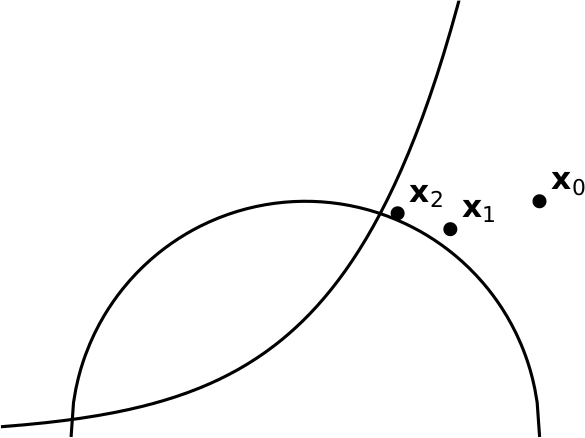
\includegraphics[width=\textwidth]{newtonexample.png}
\end{column}
\end{columns}
\end{frame}

\end{document}

